\hypertarget{backgrounds}{\chapter{Backgrounds}}

\begin{epigraphs}
\qitem{``There are two ways of constructing a software design; one way is to make it so simple that there are obviously no deficiencies, and the other way is to make it so complicated that there are no obvious deficiencies. The first method is far more difficult.''}{C. A. R. Hoare}
\qitem{``Beware of bugs in the above code; I have only proved it correct, not tried it.''}{Donald Knuth}
\end{epigraphs}

\section{Improving software dependability}
Dependability (of which security is a special case) has become more and more important of late. The definition of dependability has been given in the introduction, so we will now focus on how to create dependable software. There are many approaches on how to create dependable software; we will list those we consider to be the most important. Please note that the proposed solutions are not mutually exclusive, in fact some of them have already been combined \cite{hohmuth03applying,hunt05singularity}.

\subsection{Safe language}
A lot of software errors are not due to incorrect designs, but due to incorrect programming. The most well known problem is probably that of a \textsl{buffer overflow}. Two of the most used languages, C and C++, offer no inherent protection against buffer overflows and are thus vulnerable to this type of memory error. A solution is to design a language that is memory safe, which means that no buffer overflows can occur. Examples of these languages are C\# and Java. The problem with these languages is that they offer no fine-grained control over memory (de)allocation, which is needed for common performance optimizations to be applied.\emptyline

As maximizing performance is still vital to many programs (such as device drivers, computer games or kernels), these safe languages are often not an option. The approach taken by Cornell University was to develop a dialect of C, named Cyclone \cite{jim02cyclone}, which preserves its syntax and semantics, but also prevents some of the most common errors in the C language (such as the aforementioned buffer overflow) by using new (albeit very similar) syntax.\emptyline

Another approach is to define a completely new, safe language. This approach is taken by the John Hopkins University in their Coyotos project \cite{hopkings06coyotos}. They have developed a safe language, called BitC \cite{shapiro06bitc}, with fully specified semantics. Their approach is directly related to the next solution for a dependable system: code verification.

\subsection{Code verification}
One of the most rigorous methods to improve the dependability of software is to verify its correctness. Verification of code is done by first creating a specification of the code in a verification language and then use that language's verification capabilities to verify the required properties\footnote{An example of such a property is requiring that the program always terminates.}. Examples of verification languages, which are specifically tailored to constructing proofs, are PVS \cite{owre-pvs}, Isabelle/HOL \cite{nipkow02isabelle}, BoogiePL \cite{deline05boogiepl} and Abstract Machine Notation \cite{sorensen01towards}.\emptyline

The problem with specifying code in a verification language is that often no executable code can be generated from it. To still be able to prove properties of executable code, there are two options: convert the verification language to an executable language or vice versa. For both options it is of vital importance that the conversion retains the exact semantics of the source language, otherwise the proofs would not necessarily apply to the corresponding source code or the executable code might not do what the source specification said it would do. The problem with a semantics-retaining conversion is that both languages need to have a clear and well-defined semantics. Unfortunately, the widely used C++ language lacks in this area. Although attempts have been made to develop a clear and well-defined semantics for C++ (which will be discussed later in this chapter), the results so far are still lacking in their applicability to real-world scenarios. The Java language though \textsl{does} have a well-defined semantics; the LOOP compiler \cite{vandenberg01loop} proved that it was feasible to automatically convert Java to a higher-order logic. As a demonstration of its applicability to real-world code, Huisman et. al. used the LOOP compiler to successfully verify a non-trivial property of Java's Vector class \cite{huisman99case}. Unfortunately, the LOOP compiler is not yet generally applicable as it currently does not support threads\footnote{This is especially unfortunate considering the latest trend of developing multi-threaded applications, which is due to multi-processor systems becoming increasingly widespread.}.\emptyline

Even if one has verified properties of source code, it is ultimately the machine code that gets executed. Therefore, it is the machine code that ultimately has to be verified. If one assumes that the conversion from source code to machine code, which is done by the compiler, retains semantics, verification of the source code suffices. Curzon described in \cite{curzon92use} how a compiler can be verified.\emptyline

As said, conversion from certain languages (such as C++) to a verification language has proven to be very hard. An alternative to an automated conversion is to create a model of the source code in the verification language. This has two clear problems; first of all the conversion needs to be done \textit{by-hand} most of the time, which is a far more tedious and error-prone operation than automatic conversion, and secondly there can be no guarantee that proofs in the verification language apply to the source code (as the semantics of the model might not match those of the source code).\emptyline

To assist the prover\footnote{The program with which proofs are constructed in a verification language.} reason about correctness, some languages support the use of source code annotations, which can be used in the verification language. Annotation systems have been developed for a wide variety of languages, such as C \cite{david94lclint}, Java \cite{leavens99jml,hensel98reasoning} and a dialect of C\# called Spec\# \cite{barnett04spec}.

\subsection{Minimized kernel}
The most important part of an operating system (OS) is the kernel, as it handles critical OS parts such as process communication, scheduling and memory management. There are basically two different types of kernels: monolithic- and microkernels. A monolithic kernel executes all its code in the same address space in order to improve performance, whereas a microkernel tries to execute as much of its functionality in user space. A microkernel can be seen as a minimized version of a monolithic kernel. The basic requirements for a microkernel are given in \cite{liedtke95kernel}.\emptyline

Currently two types of microkernels are identified: first generation microkernels such as Mach \cite{rashid89mach} and Minix \cite{herder06minix} and second generation microkernels such as QNX \cite{hildebrand92architectural} and Fiasco \cite{hohmuth03applying}. First generation microkernels still contained code in the kernel which were not strictly necessary for executing its core tasks, second generation microkernels moved this code outside the kernel. Second generation microkernels are thus more \textit{strict} microkernels.\emptyline

Usually, a microkernel's tasks are limited to address space management, thread management and IPC. By restricting its functionality to these core concepts, a microkernel is typically much smaller than a monolithic kernel and thus less likely to contain bugs. Furthermore, the removal of many concepts from the kernel results in a system less likely to crash. Take for example the file server, a typical concept that is included in monolithic kernels (because of its importance on the performance of the kernel), but is not part of a typical microkernel. In the monolithic kernel, the file server has access to all kernel data; a crash of the file server can therefore result in a crash of the whole kernel (and thus everything running on the kernel). However, in the microkernel the file server executes in user space and cannot modify the kernel data. Therefore, a crash of the file server is not likely to crash the microkernel on which it is running.

\subsection{Isolation}
Another way to create a more dependable system is to contain processes in small, isolated spaces. When a process is isolated, it cannot do any harm to other (isolated) processes. There are two types of isolated processes: software isolated processes (SIPs) and hardware isolated processes (HIPs)\footnote{The terms SIP and HIP are taken from \cite{aiken06deconstructing}.}. In practice, many operating systems do not enforce strict process isolation, which results in a system where programs can modify other programs, with potentially very damaging results (for example a single driver's failure crashes the whole system).\emptyline

Hardware isolation of processes can be done by the OS, which limits a processes' memory access to specific pages of physical memory. The OS usually achieves this through standard hardware mechanisms, for example by running user processes in a less priviledged mode than kernel processes\footnote{On x86 processors, processes running at ring 0 are given full control of the processor and lower rings have limited access.}. The mechanism an OS typically uses to hardware-isolate processes is virtual memory. Even though virtual memory is directly supported by most processors, studies show that this form of process isolation is in fact quite costly \cite{aiken06deconstructing,mehnert02cost}.\emptyline

Software isolation depends on the software to isolate processes. The Singularity operating system \cite{hunt05singularity} is designed with software isolation in mind and also heavily uses language safety \cite{aiken06deconstructing,fahndrich06languagesupport,hunt05sealing}. In short, in Singularity each application runs in its own, private software \emph{box}, which ensures that the application can only modify data in its own box.\emptyline

Another form of software isolation is called virtualization. Normally the OS is the lowest software layer on a system, but virtualization adds another layer below the OS. Each virtualized OS thinks it has access to all hardware, but in fact hardware access is controlled by the virtualization layer. The process that manages the virtualization of hardware is often referred to as the \textsl{hypervisor}\footnote{This is a reference to the OS sometimes being referred to as a supervisor. Obviously the virtualization layer has more control than the OS, therefore the term hypervisor as it supersedes supervisor.}. Now several OSes (and its processes) can run simultaneously without interfering with each other (although the hypervisor might allow some limited and controlled communication between OSes), because the hypervisor ensures that an OS cannot access the hardware issued to another OS.\emptyline

Traditionally, virtualization of x86 processors is hard as the x86 architecture does not meet the Popek and Goldberg virtualization requirements \cite{popek74formal}. The main x86 processor manufacturers, AMD and Intel, acknowledged the problems with virtualization and have recently built extensions in their processors to support virtualization\footnote{Respestively called AMD Virtualization \cite{amd05virtual} and Intel Virtualization Technology \cite{intel05virtual}.}. The virtualization layer can now translate the \textit{difficult} OS calls to alternative, virtualization suitable calls, resulting in better virtualization performance.\emptyline

Another way to deal with the \textit{difficult} system calls is to apply paravirtualization. This means that the OS is modified to the extent that no \textit{difficult} calls will be made, therefore no processor-specific virtualization extensions have to be used. Unfortunately, OS modification is not possible for closed-source systems without their creators' explicit consent.
\section{L4 microkernel}

\subsection{Introduction}
A performance analysis of first generation microkernels, such as Mach, revealed that they failed to deliver a high performance microkernel \cite{hartig97performance}. Jochen Liedtke realized that one of the key reasons why Mach did not perform very well, was its complex IPC implementation. He then set himself to creating a microkernel specification that \textit{would} offer high performance; this resulted in the L3 microkernel specification \cite{metterhausen96l3}. The L3 specification had a small and efficient IPC specification, which indeed offered massive performance gains when compared to earlier microkernels such as Mach. However, Liedtke noted that the specification still contained concepts that could (and should) be moved out of the microkernel. The removal of these concepts resulted in the L4 specification. By definition the L4 microkernel specification is thus a second generation microkernel\footnote{As mentioned, a second generation microkernel is designed with both minimalism and performance in mind.}.\emptyline

The original L4 microkernel specification is the L4.V2 specification \cite{liedtke96reference}. When the L4 specification is referred to, one usually refers to the L4.V2 specification. However, the L4.V2 specification had some problems associated with it. One of the biggest problems was with the thread ids. The thread ids as specified in L4.V2 were found to be rather inflexible and unwieldy. Another problem was that the \emph{clans and chiefs} concept\footnote{The clans and chiefs concept was designed to enable the implementation of arbitrary security policies.} was too inefficient for most purposes. These problems (and more) were addressed in the L4.X0 specification \cite{liedtke99reference}. The main goal of this specification was not to solve all problems of the L4.V2 specification, but to use it as an experimental test-case. The aim of the L4.X2 release \cite{liedtke04reference} though \textsl{was} to solve the problems in the L4.V2 specification. Some of the more notable differences between the L4.V2- and L4.X2 specifications are: the separation of task- and thread management, support for multiprocessing and a clear separation between API\footnote{Application Programming Interface. The API is the source code interface with which a computer program or library lets other programs or libraries use its services.} and ABI\footnote{Application Binary Interface. An ABI allows object code to be run without changes on any system using a compatible ABI.}. Lastly, Kauer and V{\"o}lp from the Technische Universit{\"a}t Dresden have developed the L4.Sec specification \cite{kauer05reference}, which enhances the L4 specification with security features.

\subsection{Design}
Although the L4 kernel is created with minimalism in mind, there are a couple of basic concepts that have to be in the kernel:
\begin{itemize}
	\item Address spaces
	\item Threads		
	\item Inter-process communication
	\item Mapping
	\item Scheduling	
\end{itemize}

\textbf{Address spaces}
An address space is a set of mappings from virtual- to physical memory. Address spaces form the mechanism through which task-isolation\footnote{Task-isolation is the inability of tasks to tamper with the data of other tasks without their consent.} is achieved. A flexpage is a contigous region of virtual address space.\emptyline

\textbf{Threads}
A thread is the single unit of execution. Each thread belongs to a single address space, with a predefined maximum number of threads per address space. An L4 thread is characterized by a set of registers, with the instruction pointer, stack pointer and state information being required and stored in the kernel in a structure called the thread control block (TCB\footnote{Not to be confused with Trusted Computing Base.}). \emptyline

\textbf{Inter-process communication}
The sole mechanism through which threads can communicate and exchange data is inter-process communication, which as a side-effect also increases independence between system components. IPC in L4 is always synchronous, which means that no data is exchanged unless both parties agree to. IPC is also unbuffered; the kernel does not temporarily store messages which are to be sent later. L4 offers two different types of IPC: short- and long IPC. Short IPC does not involve access of user space memory and thus cannot generate page-faults; long IPC \textit{does} access user space memory and thus has to take possible page-faults into account. Short IPC only allows a limited amount of data to be be sent, messages exceeding the short IPC limit have to be sent using long IPC. When possible, short IPC is used as it offers significant performance benefits. The IPC mechanism is also used to handle both hardware- and software- interrupts\footnote{An example of a software interrupt in L4 is a timeout.} and to map-, grant and unmap flexpages. A timeout can be set to enable (unsuccessful) IPC operations to be cancelled after a specified time.\emptyline

\textbf{Mapping}
When a page-fault is generated in a thread's address space, a notification is sent to the thread's associated pager (which can be different for each thread); that pager can then insert a memory page to resolve the page-fault. Threads can map-, grant- and unmap any of its flexpages to another thread. Mapping flexpages to another thread means that the flexpages will be shared between the mapper and the mappee. Granting a flexpage to another thread passes the control of that flexpage to the grantee, the granter afterwards cannot use the granted flexpage. The unmapping of a flexpage is the inverse operation of mapping a flexpage (it can only be invoked on mapped flexpages, not on granted flexpages). The mechanism through which this is possible is IPC, where a special IPC message is sent between the two threads involved in the memory mapping.\emptyline

\textbf{Scheduling}
The scheduling of threads in L4 is priority-based, which means that the ready thread with the highest priority is always the one to be allocated CPU-time. Each thread has a priority level (of which there are 256) and time quantum associated with it. Scheduling threads with the same priority level is done through a round-robin schedule\footnote{Round-robin scheduling lets the first thread of a list of waiting threads use the CPU for a period up to its time quantum. Should the thread not be finished when it's time quantum expires, the thread is moved to the end of the list and scheduling resumes with the first item of the list.}.\emptyline

The L4 specification also mentions the concept of a \emph{task}, but this is essentially equivalent to the concept of an address space. The main difference between a task and an address space is a conceptual one: the former focuses on the system's memory and the latter focuses on the threads running in an address space. The L4 definition of a task is the set of threads sharing an address space. Creating a new task results in the creation of an address space with one thread in it.\emptyline

As one of the L4 design goals was to implement no policies, how memory is allocated is left to the application(s) running on L4; the kernel only provides the means to allocate memory. The L4 specification specifies though that the initial address space, called $\sigma_0$, should comprise all available memory (excluding kernel-reserved memory).

\subsubsection{IPC}
As said, IPC communication is always synchronous and unbuffered. Each IPC call therefore involves exactly one sender and one receiver. L4 offers five different IPC calls: \emph{send}, \emph{receive}, \emph{wait}, \emph{reply-wait} and \emph{call}. An invocation of the send call results in the sending of a single message, after which the invoker continues his work. Invoking the receive call results in the invoker waiting to receive a message from \textit{any} sender. The wait call does the same as the receive call, but only accepts messages from a single, specified sender. The last two calls are basically predefined combinations of the aforementioned calls, where each combination reflects a common real-world scenario. The call method results in the sending of a message after which the sender waits for a return message from the receiver it just sent the message to. The reply-wait operation is one in which a single message is sent after which the invoker waits for a reply from any source.\emptyline

A real-world example in which both the call- and reply-wait operations are used is a webserver. The webserver handles a request from a client, returns the results to the client and is then ready to receive a request from any client; this is equal to the reply-wait operation. From the perspective of the client, a call operation is done as the client subsequently requests data from the webserver and waits for a response from that same webserver.\emptyline

For performance guarantees, the L4 specification requires that the transitition between the send- and receive states in a single IPC call requires no time\footnote{This also protects the receiver (server) against Denial Of Service attacks.} (also referred to as an atomic switch). Having an optimized path for frequently used situations clearly benefits the system's real-world performance. Another result of combining the send and receive operations in the call and reply-wait methods is that it saves system calls (without the call method, both a send- \textit{and} receive call would have to be made to achieve the same result). As Liedtke showed in \cite{liedtke93improve}, the switching between user- and kernel mode as the result of a system call is very expensive. In both combined calls a single system call is saved, which helps to improve IPC performance.

\subsection{Implementations}
The original L4 implementation by Jochen Liedtke, sometimes referred to as L4/x86, was completely written in assembly language to maximize performance. Writing a program in assembly language has some obvious disadvantages, of which poor readability- and maintainability are probably the most important ones. Therefore, and because of licensing issues, the Technische Universit{\"a}t Dresden developed an L4-based kernel in C++ named Fiasco, which demonstrated that an implementation of the L4 specification in a higher-level language was feasible. Apart from implementing the L4 specification, Fiasco also offers hard real-time support (which is not part of the L4 specification). Similarly, Jochen Liedtke and his team at the University of Karlsruhe developed L4Ka::Hazelnut, once again as proof that an L4 microkernel could be implemented in a higher level language and still offer high performance.\emptyline

Up until this point, all L4 implementations were inheritly bound to the underlying architecture \cite{liedtke95kernel}. This changed with the advent of the L4.X2 specification. One of the first implementations of the L4.X2 specification was also developed at Karlsruhe and was named L4Ka::Pistacchio. The main aim of Pistacchio was on both performance \textit{and} portability. The new portability demand was clearly met by Pistacchio, as the supported platforms included Alpha-, ARM-, IA32-, MIPS- and PowerPC architectures. A relatively new specification and implementation originates from the National ICT Australia group. They have developed an L4 version specifically aimed at embedded systems called NICTA \cite{nicta05embedded}. 

\begin{table}[ht]
\begin{tabular}{l|l|p{20em}}
Implementation & Versions & Architectures \\
\hline
NICTA::Pistachio-embedded & N1, N2 & IA-32, ARM, Mips64 \\
L4Ka::Pistacchio & X2 & IA-32, IA-64, ARM, AMD64, PowerPC-32, PowerPC-64, Alpha, Mips64 \\
L4Ka::Hazelnut & X0 & IA-32, ARM \\
Fiasco & V2, X2 & IA-32, ARM, AMD64, UX \\
L4/x86 & V2, X0 & IA-32 \\
\end{tabular}
\caption{Overview of several L4 implementations}
\end{table}


\section{Fiasco}

\subsection{Introduction}
The Fiasco kernel is based on the aforementioned L4 specification. Fiasco is a second generation microkernel, which means that it is created with minimalism (nothing exists in the kernel that cannot be moved out of it) and performance in mind. The effect of minimalism can clearly be seen in the number of lines of code the kernel comprises: around 20.000 lines of code for Fiasco compared to around 3.2 million for the Linux kernel. The Fiasco kernel is developed with real-time features in mind, which means that the system is fully preemptable\footnote{Execution can be interrupted at almost any time, which means the work is temporarily halted in favor of (at that moment) higher priority work. After the prioritized work has finished, the system continues with the interrupted execution.}. 

\subsection{History}
DROPS\footnote{Dresden Real-time OPerating Systems project.} \cite{hartig98drops} is a research project which aims to find design techniques to implement a distributed, real-time operating system where every component can guarantee a certain level-of-service to applications. The foundation of DROPS is based on the L4 specification. As the original L4/x86 implementation by Jochen Liedtke had some serious disadvantages (readability, maintainability and licensing issues), the Technische Universit{\"a}t Dresden decided to create their own implementation of the L4 specification, called Fiasco, which could be used by DROPS. Besides implementing the L4.V2 and L4.X2 specifications, Fiasco sets itself apart from other L4 implementations with its real-time features, obviously created with DROPS' real-time focus in mind.\emptyline

Another project related to Fiasco is Fiasco-UX \cite{schonberg01user}, which is a port of the Fiasco microkernel to the Linux system-call interface. This means that Fiasco-UX can be run as an application on a Linux system and due to its special design (no need for kernel-level priviliges) it can even be run as a regular user-level application. One of the main benefits of this approach is its ease of use, particularly when developing applications for Fiasco. Rebooting the machine due to a (kernel) crash is no longer necessary, a simple restart of the Fiasco-UX process suffices. Another advantage is that several instances of Fiasco-UX can run in parallel.\emptyline

We will now discuss in more detail the features of Fiasco that are relevant to our research.

\subsection{Threads}
Besides implementing the L4 thread specification, Fiasco also implements some additional mechanisms for performance- and real-time support purposes. Some of the performance optimizations stem from \cite{liedtke93improve}.

\subsubsection{Scheduling}
As the L4 specification dictates, a thread has properties such as a time quantum and priority associated with it; these properties of a thread are called its \emph{scheduling context} and are used in the scheduling of threads. To support the real-time features of Fiasco, each thread can also have an additional real-time scheduling context\footnote{This is not part of the L4 specification.}. An \emph{execution context} is a runnable, schedulable thread. At all times there is only one active execution context (or thread), as Fiasco does not support multi-processor execution (it will only use one of the processors available). A thread's current state of execution is stored in its thread control block (TCB), which resides in the kernel. Switching execution of threads can therefore be done through a simple TCB switch. The scheduler uses the \emph{ready-list} (containing all threads ready to be run) to decide what thread to run next. More details on scheduling in Fiasco can be found in \cite{steinberg05quality}.

\subsubsection{Ready-list}
As said, the system keeps a list of all threads ready to be executed: the ready-list. Although it might seem odd at first, the ready-list can contain threads that are \textit{not} ready to be executed. If the scheduler finds such a thread while traversing the ready-list, it is immediately removed from it. The goal of this \emph{lazy-scheduling} is improving the performance of IPC. As an example, we look at a call to the \emph{call} IPC function, in which a sender sends a message to a receiver and then waits for that receiver to send a message back. If we were to strictly adhere to the property that the ready-list only contains ready threads, this IPC call would result in the following modifications to the ready-list:

\begin{itemize}
 \item After the sender has sent its message, the sender enters a waiting mode and has to be dequeued.
 \item After the sender has sent its message, the receiver becomes ready and has to be enqueued.
 \item After the receiver has sent its message, the receiver enters a waiting mode and has to be dequeued.
 \item After the receiver has sent its message, the sender becomes ready and has to be enqueued.
\end{itemize}

We see that this common scenario results in four different changes to the ready-list. Obviously, this is detremental to IPC performance. However, if we allow non-ready threads in the ready-list and exclude the current executing thread from it (which is ready by definition), all four modifications can be saved. After the sender has sent its message, the receiver does not need to be enqueued as it has become the current executing thread. Similarly, once the receiver has sent its message back, the sender does not need to be enqueued as it will be the currently executing thread. Both dequeue actions can be saved as we allow threads in the ready-list that are not ready, which is precisely what entering a waiting mode signifies. To successfully apply this lazy-scheduling, the kernel has to make sure that the current executing thread will be enqueued in the ready-list if it cannot finish its task within its timeslice. If we would leave out this clause, the current executing thread is not guaranteed to get scheduled again (remember that it is not contained in the ready-list while executing), which is necessary in order to finish its task.\emptyline

To switch execution from sender to receiver (and vice versa) without ready-list scheduling, the system uses their execution contexts. Say we want to switch execution from thread A (which is the current active thread) to thread B, but without using the ready-list. To do so, a simple switch of execution context from A to B suffices, as the current execution context determines what is executed. It is not necessary to also switch the scheduling context from A to B, in fact it is better not to for the following reason. If the scheduling context is not changed when the execution context is switched, thread B gets to execute as if it were A, which means that it can execute for the remainder of A's timeslice. This optimization gives B more execution time than it would normally have, thereby allowing it to finish sooner. In our \emph{call} example, this means that after the sender has sent its message, an execution switch is made to the receiver which gets to execute in the sender's timeslice. Therefore, it is likely that the receiver is able to send a message back sooner, as the sender's timeslice remainder would otherwise be wasted by waiting on the receiver.\emptyline

In some situations, it might not be useful to immediately switch to the receiver but instead enqueue the receiver in the ready-list (which is the normal way in which a thread gets to execute). For this situation the \emph{deceit-bit hack} can be used. Originally, the deceit-bit was used in the L4 clans \& chiefs concept, but as this concept proved too inflexible it is almost never implemented. Therefore, the deceit-bit was \textit{free} for other purposes and in Fiasco it is used to signal that no lazy-scheduling should be applied.

\subsection{Synchronization}
Having a fully preemptable system requires some form of synchronization for critical parts. Fiasco supports two different types of synchronization: \emph{lock-free}- and \emph{wait-free} synchronization. The main difference between the two synchronization types is in their intended use: lock-free synchronization should be used for time-critical synchronization (such as the synchronizing of frequently accessed, global data) and wait-free synchronization should be used for non time-critical operations (such as the synchronizing of local data). The two synchronization types are implemented as follows:

\begin{itemize}
	\item Lock-free synchronization: this is achieved through atomic updating of memory\footnote{The x86 processor provides the compare-and-swap (CAS) instruction for exactly this purpose.}. It tries to exchange old data for new data and if this fails it simply retries. In order to prevent the system from retrying infinitely (which would invalidate the real-time properties of the system), a specific retry-count can be set. While setting the data, interrupts will be temporarily disabled to prevent another thread from modifying the data.
	\item Wait-free synchronization: this is a locking-type of synchronization, in which exclusive access to resources can be obtained by creating a lock. Fiasco expands on this well-known mechanism by introducing \emph{switch locks} (also referred to as \emph{helping locks}). Suppose thread A has locked a resource X which thread B also wants to access. Normally, B would just use up all of its execution time waiting on A to release the lock on X. However, instead of wasting execution time on waiting, B can also help A release its lock sooner by donating its remaining timeslice to A. Now A has more execution time available and will likely release the lock on X sooner, which is exactly what B wants. One might note the similarity of this optimization to the thread switch optimization in the ready-list description.
\end{itemize}

A full description of the design philosophy and implementation of these two synchronization mechanisms can be found in \cite{hohmuth01pragmatic}.

\subsection{Locks}
Wait-free synchronization in Fiasco can be achieved through the use of locks. Basically there are two types of locks: regular- and switch locks. Of the former there exists just one in Fiasco, namely the CPU lock, which temporarily disables interrupts. This lock should only be used for very short intervals as it can negatively influence the real-time features of the system. The other two locks in Fiasco are switch locks. The first switch lock is the thread lock, which locks access to a thread. The second switch lock is the helping lock, which is similar to the switch lock save from the fact that it also works when the scheduling system has not yet been loaded.\emptyline

Switch locks are designed explicitly with IPC performance in mind; its basic optimization principle strongly resembles that discussed in the ready-list discussion. The implementation is as follows. When the current thread tries to acquire a lock on a resource by using a switch lock but detects that the resource is already locked, the lock count of the current thread is incremented. After incrementing the lock count, the switch lock keeps on switching to the lock owner (by switching the execution context to that of the lock owner) until the lock is free and can be acquired. Afterwards, when the lock is released, the lock count is decremented and the lock checks if it has been helped by another thread (which donated execution time to the thread holding the lock), if so it switches the execution context to that of the helper.\emptyline

When a thread is locked, it will not be selected by the scheduler. Should a switch be made to a locked thread, the system will immediately switch to that thread's lock owner. Although locked threads normally do not get scheduled, an exception arises when a thread is killed. A thread that is to be killed should hold no locks at all, therefore the system keeps scheduling such a thread until it has released all its locks. The thread's lock count is used to determine if any locks are still present.

\subsection{Timeouts}
Fiasco recognizes three different types of timeouts: IPC-, deadline- and timeslice timeouts. An IPC timeout is used to restrict an IPC call to a specific maximum time, which can be used to prevent senders and receivers from waiting endlessly on each other. A deadline timeout is used to set timed deadlines and a timeslice timeout is used to signal the end of a timeslice.\emptyline

Internally, timeouts are stored in a list that is ordered in ascending timeout order (the head of the list is the oldest timeout and the first to occur). When the system checks if timeouts occured, the timeout list can thus be traversed sequentially. Therefore, detecting timeouts is very fast whereas enqueuing or dequeuing is rather slow. For more details on the implementation of timeouts see \cite{reusner05impl}.

\subsection{IPC}
IPC in Fiasco supports all L4 IPC calls, namely \emph{send}, \emph{receive}, \emph{wait}, \emph{reply-wait} and \emph{call}. All these functions are internally supported through one generic function: \emph{sys\_ipc()}, which parameters determine the actual call made. We will now describe the general setup of IPC in Fiasco.

\subsubsection{Sender and receiver roles}
IPC in Fiasco is synchronous and thus always involves a single sender- and receiver communicating (sending messages) with each other. In Fiasco, there are separate definitions for the sender- and receiver roles. As threads need to both send- \textit{and} receive messages, they extend (inherit from) both the receiver- and the sender role. In Fiasco, only threads extend the receiver role, in other words only threads can receive IPC messages. However, there are two more objects extending the sender role, namely the IRQ and preemption objects. The first translates hardware interrupts into IPC messages, which demonstrates the very generic applicability of Fiasco's receiver/sender setup. The second sends messages dealing with preemptions. As both the IRQ and preemption objects can only send messages (as they do not extend the receiver role), they are also known as \emph{passive senders}.\emptyline

\begin{figure}[ht]
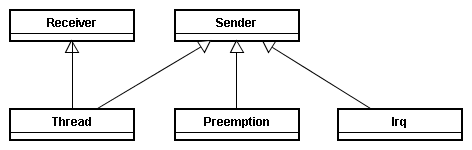
\includegraphics[scale=0.50]{images/diagrams/ipc_class_ipc_roles}
\caption{Fiasco IPC roles diagram.}
\end{figure}

Due to IPC's synchronous nature, a receiver can only receive a message from a single sender. As it is possible that a receiver is unable to directly engage in IPC with a sender (for example because it is already engaged in IPC with another sender), the receiver should be able to queue send requests. This is achieved in Fiasco by letting the receiver have a sender list, which is a list of senders wanting to send a message to the receiver. Once a receiver engages in IPC with a sender, that sender is removed from the sender list (if he was it in).\emptyline

When an IPC call is made, the transferring of a message is handled from the viewpoint of the sender, it is the sender that determines which actions to do first and how to continue. An exception to this situation occurs when the sender is a passive sender; in this case the receiver controls IPC.

\subsubsection{IPC overview}
Although there are five different IPC calls, internally there is only one function that handles IPC: \emph{sys\_ipc()}. IPC (and thus the \emph{sys\_ipc()} function) can be divided into a send and receive part. Obviously, the send part handles the sending of an IPC message and the receive part handles the receiving thereof. The table below lists what IPC parts are involved in the five IPC calls:

\begin{table}[ht]
\begin{tabular}{l|l|p{20em}}
IPC call & Send part & Receive part \\
\hline
\emph{send} & x & - \\
\emph{receive} & - & x \\
\emph{wait} & - & x \\
\emph{reply-wait} & x & x \\
\emph{call} & x & x \\
\end{tabular}
\caption{Mapping of L4 IPC calls to Fiasco send and receive parts.}
\end{table}

The following schema gives an overview of how the send and receive parts are handled in Fiasco:

\begin{figure}[ht]
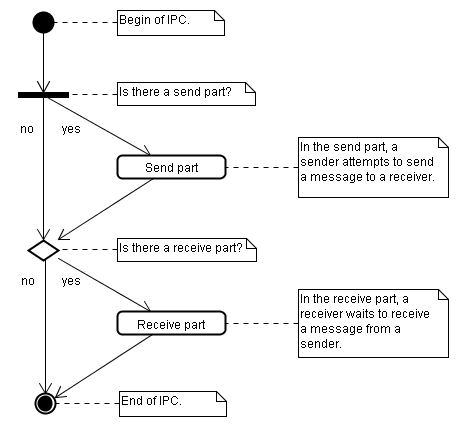
\includegraphics[scale=0.50]{images/diagrams/ipc_activity_ipc_overview}
\caption{IPC overview.}
\end{figure}

One might remember that in the \emph{reply-wait} and \emph{call} calls, the message sending preceded the receiving of a message. In Fiasco, the receive part is handled \textit{after} the send part to allow the aforementioned two calls to be handled in a single execution of the IPC path (this sequential structure has no influence on the functionality of the other three IPC calls).\emptyline

Before a message can be sent in the send part, the sender and receiver have to agree upon engaging in IPC; this is referred to as the \emph{handshake}. It is possible that the receiver is not immediately ready to receive a message from the sender, for example because it is still engaged in IPC with another sender; in that case the sender is added to the receiver's sender list and waits for the receiver to become ready. If an error occured in the handshake, IPC is aborted. However, if the handshake was successful, the sender can then send its message to the receiver. The following schema displays this set-up:

\begin{figure}[!ht]
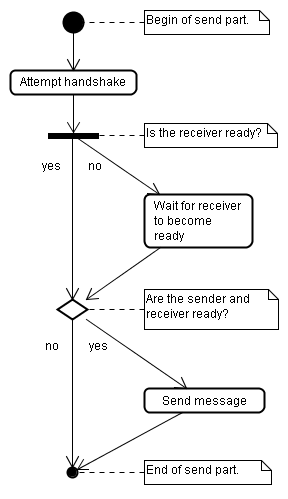
\includegraphics[scale=0.50]{images/diagrams/ipc_activity_send_part}
\caption{IPC send part overview.}
\end{figure}

As control of IPC is mostly handled by the sender (and thus in the send part), the receive part does relatively little. What \textit{is} done in the receive part is that the receiver enters a loop. With each iteration, it checks if it is ready to receive a message and if there is a sender that wants to send a message (which is indicated by a non-empty sender list). If there is such a sender, the receiver sends it a signal to indicate that it is ready to receive a message. That sender is subsequently removed from the sender list by the receiver. Only when the receiver is not ready to receive a message is the receive part aborted.

\begin{figure}[!ht]
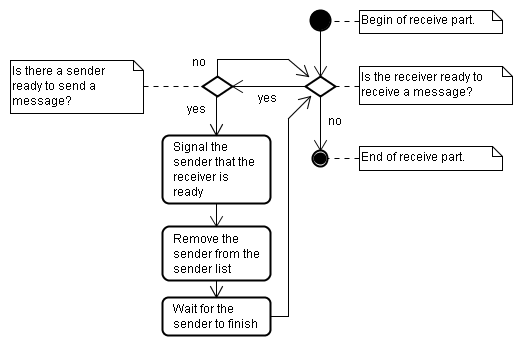
\includegraphics[scale=0.50]{images/diagrams/ipc_activity_receive_part}
\caption{IPC receive part overview.}
\end{figure}

\subsubsection{IPC paths}
Because IPC in Fiasco is unbuffered, no messages are temporarily stored by the kernel; instead messages are transferred directly between sender and receiver. As described in the L4 specification, Fiasco discerns between three different message types: untyped data (direct strings), memory-buffer references (indirect strings) and memory mappings (flexpages).\emptyline

There are two paths in Fiasco through which an IPC message can be transferred: a short- and long IPC path. 
\begin{itemize}
  \item Short IPC path: this path uses only the system registers for transferring messages. The size of the data which can be transferred is thus limited to the size of the available registers. The advantages of only using the system registers for message transfer are that it is very fast and that no page-faults can occur (as no user-space memory is accessed). As an example of where the short IPC path is put to good use, when a page-fault IPC message is sent to a pager, that pager should respond with a flexpage IPC message to resolve the page-fault. Because a single flexpage does not exceed the size of the registers, it can be sent using the short IPC path allowing for a fast response by the pager. Secondly, when a direct string is sent, the system puts as much of that direct string into the registers; if the direct string does nog fit completely into the registers, the rest of the direct string is transferred using the long IPC path.
  \item Long IPC path: all message types can be transferred through the long IPC path, that includes indirect strings. Where the short IPC path limits the sending of flexpages to a single value, the long IPC path can send several flexpages at once. The transferring of messages is done by creating an IPC window. The IPC window is a part of the receiver's address space, which is mapped to the sender's address space during the message transfer. The sender can now directly copy the messages into the address space of the receiver, which prevents the kernel from buffering the messages. The main disadvantage of long IPC is that it has to invoke user-space memory, which could generate page-faults. A generated page-fault is sent to the pager of the receiver, as it is the receiver's address space that is being written to. Also, the long IPC path is slower than the short IPC path.
\end{itemize}

\subsubsection{IPC shortcut path}
Besides the two aforementioned IPC paths, there is also an IPC shortcut path. Basically, the IPC shortcut is an alternative version of the short IPC path (it thus also transfers messages through the system registers), but with some further restrictions applied to it (which enable performance optimizations). One of the restrictions of the shortcut is that it does not support the receive- and wait calls. Another restriction is that a single flexpage cannot be sent using the shortcut, only direct strings which fit into the registers are thus eligible for use with the IPC shortcut. Furthermore, the supported timeouts are limited to zero- (immediate response required) and infinite (no time-out at all) timeouts. The IPC shortcut completely runs with interrupts disabled. \emptyline

The reason why the IPC shortcut was developed is simple: most of the system calls are IPC calls and most of the IPC messages are short IPC messages. Therefore, when the transfer of these short messages is optimized, the performance of the whole system is likely to improve significantly. There are two different versions of the shortcut. The normal version is implemented in C++, but there is also an optimized version of the shortcut, which is written in assembler and has been developed by Michael Peter \cite{peter02leistung}.

\subsubsection{IPC states}
The state of an IPC operation is stored at the receiver; this state is stored as a bit mask in which each bit corresponds to a specific state the thread can be in (for example waiting for a receiver or sending an IPC message). There are several functions to modify the state, which can add-, delete- or at once add- and delete bits in the state. These functions are respectively \emph{state\_add()}, \emph{state\_del()} and \emph{state\_change()}. All these functions are atomic operations, which means that they are guaranteed to succeed. The disadvantage of these atomic operations is that they are unnecessarily expensive when interrupts are already disabled. In this case regular operations would have exactly the same result as they too are then guaranteed to succeed, but without incurring the performance penalty of atomic operations. Fiasco therefore offers non-atomic variants of the state modification functions which are suffixed with "\_dirty" (leading to the \emph{state\_add\_dirty()}, \emph{state\_del\_dirty()} and \emph{state\_change\_dirty()} functions). Please note that these \textit{dirty} functions assume that interrupts are disabled, they do not check this themselves; it is therefore the responsibility of the caller to make sure interrupts are disabled when calling these functions.

\subsubsection{Priority inversion}
One of the classic scheduling problems is priority inversion, where a lower priority task is prioritized over a higher priority task. This situation occurs when a lower priority task has locked a shared resource that a higher priority task also wants to access. The higher priority task has no choice but to wait for the lower priority task to release the lock; the priorities are thus temporarily inversed. In Fiasco's old IPC path this problem existed when a combined send- and wait call was made. Let us consider a situation in which a sender A is engaged in a combined send- and wait operation with receiver B. As soon as A has sent its message to B, sender A enters a waiting state and an immediate execution context switch is made to receiver B (this optimization is described in the ready-list section). Because the receiver B gets to execute in the scheduling context of A, it will temporarily inherit the priority of A. Now suppose just before the switch to B, a second sender (which we call C) tries to send a message to B. If the priority of C is less than or equal to the priority of A, there is no problem. However, when C has a higher priority than B, the switch from B to A (which has B's priority) violates the priority-based scheduling invariant\footnote{Which states that higher priority threads should always be scheduled before lower priority threads.}.\emptyline

This problem was fixed in the current IPC implementation; its solution was actually quite simple: before switching to the receiver, the sender should check if there is a sender with a higher priority than its own that wants to send a message to the same receiver. Should this be the case, the receiver is added to the ready-list and the system switches to the higher priority sender. If no other higher priority sender exists, the immediate switch to the receiver can be done without any problem.

\subsubsection{Real-time features}
Because IPC is of vital importance to the performance of Fiasco (in fact, it is of vital performance to \textit{any} microkernel), improving IPC is thus one of the key performance improving strategies. However, with Fiasco a constant eye has to kept at the real-time features of the system. Often, there is a trade-off between performance and real-time support. This can clearly be seen in Ren\'e Reusner's attempt to improve the performance of IPC in Fiasco, which includes clear graphs detailing the trade-off results \cite{reusner05impl}.\emptyline

Probably the best example of such a performance versus real-time features trade-off is the decision on which parts of the IPC path should be non-interruptible. If one makes the IPC path non-interruptible, this prevents the use of synchronization mechanisms, which are required in an interruptible path and thus improves performance. The real-time features are invalidated though. The current IPC path is non-interruptible in the following phases: the setup, rendez-vous and finish phase. Furthermore, when sending direct strings in the register transfer (short IPC) phase, the system remains non-interruptible. However, when a flexpage is sent in the register transfer phase or the memory transfer phase is used, the system \textit{is} interruptible. An interruptible path has good real-time features, but this comes at the cost of decreased performance.\emptyline

Although most phases are non-interruptible, in- and between phases interrupt points and -regions have been inserted to preserve the real-time features. An interrupt region is created by calling \emph{Proc::sti()} (enable interrupts) at the beginning- and \emph{Proc::cli()} (disable interrupts) at the end of the region. An interrupt point is created by calling the \emph{Proc::preemption\_point()} function\footnote{Internally, this function first enables interrupts by calling \emph{Proc::sti()}, than executes the \emph{nop()} instruction (which does not do anything) twice to give interrupts the chance and then disables interrupts again by calling \emph{Proc::cli()} after which it returns.}. Please note that there also is a preemption point at the very beginning of an IPC operation, before the \emph{sys\_ipc()} function is called. The disadvantage of using interrupt points and -regions is that additional checks are needed because the state might have changed while interrupts were allowed.

\begin{figure}[ht]
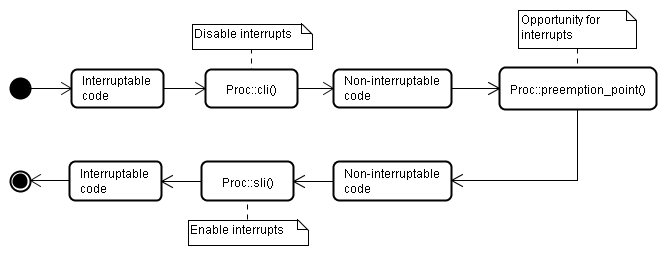
\includegraphics[scale=0.50]{images/diagrams/ipc_activity_interrupts}
\caption{Fiasco interrupt transitions.}
\end{figure}
\section{PVS}

\subsection{Introduction}
PVS stands for Prototype Verification System and has been developed by SRI International, an independent, non-profit research institute \cite{sri06nonprofit}. The PVS language is a simply typed, higher-order logic language. The language offers built-in types such as booleans and integers, but also supports custom defined types. There are several type-constructors available, ranging from functions to enumerations. PVS also supports (and includes) inductively defined data types such as lists and binary trees. To help in creating proofs, PVS by default supplies the user with many lemmas that can be used in creating a proof\footnote{An example is the lemma \emph{reverse\_reverse}, which states that reversing a list twice results in the original list.}.\emptyline

In PVS, specifications can be written just like in any regular functional language. Specifications are however not created to generate an executable, but with the goal of proving properties of those specifications. PVS thus cannot be used directly to create a provably correct program, but it could create a provably correct program specification \cite{miller95formal}. Having a provably correct program specification is particularly useful when designing a life-critical application\footnote{We define a life-critical application as one where a failure in the application might result in the loss of one or more lives.} such as the software running a space shuttle. In fact, NASA has been using PVS for it's space shuttle program \cite{crow98formalizing} and has actively participated in PVS-related research \cite{vito03application}.\emptyline

The PVS theorem prover lies at the heart of every proof in PVS; it has a predefined collection of inference procedures which the user can apply interactively within a sequent calculus framework. Examples of inference procedures are rewriting, simplifying and applying induction. There are also predefined proof strategies, which are essentially just combinations of the inference procedures. PVS also allows the user to create his or her own strategies.\emptyline

For those unfamiliar with sequent calculus, a short description will now follow. The objective of a proof is to generate a proof tree of \emph{sequents} in which all leaves are trivially true. Each node of a proof tree is such a sequent. A sequent is a combination of \emph{antecedents} and \emph{consequents}. Sequents are interpreted such that the conjuction of the antecedents implies the disjunction of the consequents. Less formally, the antecedents are what is assumed to be true and the consequents are what one wants to prove to be true.

\subsection{Features}
We will now discuss some of the more noteworthy PVS features which have found their way into our research.

\subsubsection{Theory importing}
Every declaration (such as lemmas, functions or types) defined in PVS belongs to a single, named theory. For ease of use, it is possible to have one theory import other theories (as long as there are no circular references), which definitions can then be used. This allows one to create modular theories, where general purpose declarations can be defined once and used more than once.

\subsubsection{Extensible records}
From PVS version 4.0 and up, the concept of extensible records has been introduced into PVS. This concept allows one record to extend another record. This means that when a record extends another record, it automatically contains (or inherits) all fields defined in the record which it extends. This mechanism can be used to define a simple type of inheritance. The example below shows three record types: \emph{record1} is a regular record type, but \emph{record3} inherits from the \emph{record2} by using the extensible records concept. The result of the extension is that the \emph{record1} and \emph{record3} types are equal (they have exactly the same fields), although they have used different methods to achieve this.

\lstset{language=PVS}
\begin{lstlisting}[caption={PVS: example of the extensible records mechanism.}]
% record1 does not inherit any fields, it defines them all itself.
record1: TYPE = [# a: type_a, b: type_b #]

% Have record3 inherit all fields from record2, this results in record3 having exactly
% the same fields as record1.
record2: TYPE = [# a: type_a #]
record3: TYPE = record2 WITH [# b: type_b #]
\end{lstlisting}

\subsection{Example proof}

% The following substitutions are from the file:
%   /usr/local/pvs-4.0/pvs-tex.sub
\def\setsotherremovetwofn#1#2{{(#2 \setminus \{#1\})}}% How to print function sets.remove with arity (2)
\def\setsotheraddtwofn#1#2{{(#2 \cup \{#1\})}}% How to print function sets.add with arity (2)
\def\setsotherdifferencetwofn#1#2{{(#1 \setminus #2)}}% How to print function sets.difference with arity (2)
\def\setsothercomplementonefn#1{{\overline{#1}}}% How to print function sets.complement with arity (1)
\def\setsotherintersectiontwofn#1#2{{(#1 \cap #2)}}% How to print function sets.intersection with arity (2)
\def\setsotheruniontwofn#1#2{{(#1 \cup #2)}}% How to print function sets.union with arity (2)
\def\setsotherstrictunderscoresubsetothertwofn#1#2{{(#1 \subset #2)}}% How to print function sets.strict_subset? with arity (2)
\def\setsothersubsetothertwofn#1#2{{(#1 \subseteq #2)}}% How to print function sets.subset? with arity (2)
\def\setsothermembertwofn#1#2{{(#1 \in #2)}}% How to print function sets.member with arity (2)
\def\opohtwofn#1#2{{#1\circ#2}}% How to print function O with arity (2)
\def\opdividetwofn#1#2{{#1/#2}}% How to print function / with arity (2)
\def\optimestwofn#1#2{{#1\times#2}}% How to print function * with arity (2)
\def\opdifferenceonefn#1{{-#1}}% How to print function - with arity (1)
\def\opdifferencetwofn#1#2{{#1-#2}}% How to print function - with arity (2)
\def\opplustwofn#1#2{{#1+#2}}% How to print function + with arity (2)
As a short example of creating a proof in PVS, we will prove that the square of any odd number is also an odd number. This corresponds to the following lemma in PVS:\emptyline

\pvsid{odd\_square\_is\_odd}: \pvskey{LEMMA}
    \(\forall\) \pvsid{(}\pvsid{number}: \pvsid{int}\pvsid{)}: \pvsid{odd?}\pvsid{(}\pvsid{number}\pvsid{)} \(\implies\) \pvsid{odd?}\pvsid{(}\(\optimestwofn{\pvsid{number}}{\pvsid{number}}\)\pvsid{)}\vspace*{\pvsdeclspacing}\emptyline

In this lemma, we use {\pvsid{odd?}}, which is only true if the supplied argument is an odd number in PVS (the definition of odd? can be found in the PVS prelude). When we start proving this lemma, we are initially presented with the following sequent:\emptyline

\begin{tabular}{|cl}
\strut\\\hline
$\{\mbox{\rm 1}\}$ &\begin{minipage}[t]{5.5in}{\begin{alltt}\(\forall\) \pvsid{(}\pvsid{number}: \pvsid{int}\pvsid{)}: \pvsid{odd?}\pvsid{(}\pvsid{number}\pvsid{)} \(\implies\) \pvsid{odd?}\pvsid{(}\(\optimestwofn{\pvsid{number}}{\pvsid{number}}\)\pvsid{)}\end{alltt}}\end{minipage}\\
\end{tabular}

\vspace{0.1in}

As can be seen, we now have one consequent (the formula numbered 1, appearing below the line) that corresponds to the statement we want to prove. Currently, this consequent deals with \textit{any} possible number (referred to as a universal quantifier), but we want to limit it to a single instance (or constant) for easier proof creation. To replace the universal quantifier with a constant, we issue the \pvscmt{(skolem!)} command.\emptyline

\begin{tabular}{|cl}
\strut\\\hline
$\{\mbox{\rm 1}\}$ &\begin{minipage}[t]{5.5in}{\begin{alltt}\pvsid{odd?}\pvsid{(}\(\pvsid{number}'\)\pvsid{)} \(\implies\) \pvsid{odd?}\pvsid{(}\(\optimestwofn{\pvsid{number}'}{\pvsid{number}'}\)\pvsid{)}\end{alltt}}\end{minipage}\\
\end{tabular}

\vspace{0.1in}

The result is now that the universal quantifier has been replaced by a constant. In the rest of our proof, we will use this constant.\emptyline

For our proof, we need an antecedent stating that {{\pvsid{number}\('\)}} is an odd number. At the moment, this assumption is still contained in the formula in consequent 1. To remedy this, we apply the \pvscmt{(flatten)} command.\emptyline

\begin{tabular}{|cl}
$\{\mbox{\rm -1}\}$ &\begin{minipage}[t]{5.5in}{\begin{alltt}\pvsid{odd?}\pvsid{(}\(\pvsid{number}'\)\pvsid{)}\end{alltt}}\end{minipage}\\\hline
$\{\mbox{\rm 1}\}$ &\begin{minipage}[t]{5.5in}{\begin{alltt}\pvsid{odd?}\pvsid{(}\(\optimestwofn{\pvsid{number}'}{\pvsid{number}'}\)\pvsid{)}\end{alltt}}\end{minipage}\\
\end{tabular}

\vspace{0.1in}

The result of the \pvscmt{(flatten)} command is that the odd number assumption has been removed from consequent 1 and added as antecedent -1.\emptyline

To be able to continue our proof, we have to look at how odd numbers are defined in PVS. To do so, we expand the definition of \pvsid{odd?} by issuing \pvscmt{(expand "odd?")}.\emptyline

\begin{tabular}{|cl}
$\{\mbox{\rm -1}\}$ &\begin{minipage}[t]{5.5in}{\begin{alltt}\(\exists\) \(j\): \(\pvsid{number}'\) \(=\) \(\opplustwofn{1}{\optimestwofn{2}{j}}\)\end{alltt}}\end{minipage}\\\hline
$\{\mbox{\rm 1}\}$ &\begin{minipage}[t]{5.5in}{\begin{alltt}\(\exists\) \(j\): \(\optimestwofn{\pvsid{number}'}{\pvsid{number}'}\) \(=\) \(\opplustwofn{1}{\optimestwofn{2}{j}}\)\end{alltt}}\end{minipage}\\
\end{tabular}

\vspace{0.1in}

Once again, quantifiers have been introduced into our proof. As we want to use the constant {{\pvsid{number}\('\)}} in consequent 1, we have to make sure there are no quantifiers in antecent -1 (in which the constant {{\pvsid{number}\('\)}} is defined). This is done by issuing the \pvscmt{(skolem!)} command again.\emptyline

\begin{tabular}{|cl}
$\{\mbox{\rm -1}\}$ &\begin{minipage}[t]{5.5in}{\begin{alltt}\(\pvsid{number}'\) \(=\) \(\opplustwofn{1}{\optimestwofn{2}{j'}}\)\end{alltt}}\end{minipage}\\\hline
$\{\mbox{\rm 1}\}$ &\begin{minipage}[t]{5.5in}{\begin{alltt}\(\exists\) \(j\): \(\optimestwofn{\pvsid{number}'}{\pvsid{number}'}\) \(=\) \(\opplustwofn{1}{\optimestwofn{2}{j}}\)\end{alltt}}\end{minipage}\\
\end{tabular}

\vspace{0.1in}

The result is that the {{\pvsid{number}\('\)}} constant is now removed of its quantifiers, which means that we can use it in consequent 1.\emptyline

At this point, we have to decide how we can use the odd number constant in antecedent -1 to prove consequent 1. For this, it is best to look at how one would verify this statement mathematically. If we look at consequent 1, we want to find a number $j$ such that:

\begin{equation}
number^\prime * number^\prime = 1 + 2 * j
\end{equation}

If we could find such as number $j$, $number^\prime * number^\prime$ would conform to the definition of an odd number (which is what we wanted to prove). We can find this number $j$ by rewriting the definition of {{\pvsid{number}\('\)}}:

\begin{equation}
\begin{split}
number^\prime & = 1 + 2 * j^\prime\\
number^\prime * number^\prime & = (1 + 2 * j^\prime) * (1 + 2 * j^\prime)\\
                & = 1 + 4j^\prime + {4j^\prime}^2\\
                & = 1 + 2 * (2j^\prime + {2j^\prime}^2)
\end{split}
\end{equation}

This simple rewrite has provided us with the value we can use for $j$:

\begin{equation}
j = 2j^\prime + {2j^\prime}^2
\end{equation}

Returning to our proof, we can use the value of $j$ we found in our proof by instantiating consequent 1. We can now initialize the quantifier in consequent 1 with the value found: \(\opplustwofn{\optimestwofn{2}{j'}}{\optimestwofn{\optimestwofn{2}{j'}}{j'}}\):\emptyline

\begin{tabular}{|cl}
$\{\mbox{\rm -1}\}$ &\begin{minipage}[t]{5.5in}{\begin{alltt}\(\pvsid{number}'\) \(=\) \(\opplustwofn{1}{\optimestwofn{2}{j'}}\)\end{alltt}}\end{minipage}\\\hline
$\{\mbox{\rm 1}\}$ &\begin{minipage}[t]{5.5in}{\begin{alltt}\(\optimestwofn{\pvsid{number}'}{\pvsid{number}'}\) \(=\) \(\opplustwofn{1}{\optimestwofn{2}{\opplustwofn{\optimestwofn{2}{j'}}{\optimestwofn{\optimestwofn{2}{j'}}{j'}}}}\)\end{alltt}}\end{minipage}\\
\end{tabular}

\vspace{0.1in}

Everything is now in place to finish the proof, which can be done by applying \pvscmt{(assert!)}.\emptyline

This completes the proof of {\tt odd\_square\_is\_odd}.\emptyline

Q.E.D.
\hypertarget{related_work}{\section{Related work}}
Although the Fiasco kernel is in continuous development, there already has been some effort in formally verifying it. In this respect, Fiasco also serves as a test project to study the feasibility of a verified microkernel. The attempts to verify the Fiasco kernel belong to the VFiasco project \cite{hohmuth03applying}. Besides describing why they want to verify the Fiasco kernel, Hohmuth and Tews also describe why they decided to verify the C++ Fiasco source and not re-implement the kernel in a 'safe' programming language. It is interesting to see that the approaches taken to verify parts of Fiasco differ on many parts.

\subsection{Verifying memory management in Fiasco}
One of the first attempts to verify the Fiasco kernel focused on Fiasco's memory management \cite{tews00case}. The approach taken by Tews was to create a co-algebraic model of memory management in Fiasco in the CCSL language \cite{hensel98reasoning}. After Fiasco's memory management was modelled in CCSL, this model was compiled to a PVS specification in which properties of the co-algebraic model were proven. The approach taken was successful in formally verifying several properties of Fiasco's memory management. There were however two problems with the approach taken. First of all, CCSL lacks support for imperative programming, which lessens its applicability to real-world situations as imperative programming is widely used. Therefore, creating a model of Fiasco (which was written in an imperative language) was not as intuitive in CCSL as it could be. The second problem was the creation of the CCSL model from the Fiasco source, which had to be done by hand. So far, no conversion can be made from C++ to CCSL, which is mainly due to the complexity of C++. This leaves one no choice but to convert the source code by hand, which can be a daunting task for large programs. A manual conversion also has the disadvantage that, strictly speaking, the properties proven only apply to the CCSL model and not to the actual C++ source. This is because one cannot guarantee that the hand-made C++ to CCSL conversion retains the source code's semantics. As said, defining a formal semantics of C++ is extremely hard due to its complexity. According to the author, this leaves us with two solutions: only verify source code in a language with well-defined semantics or use a well-behaved subset of C++ with a clear semantics.

\subsection{Developing a C++ semantics compiler}
In line with the conclusions of the work described above, development of a C++ semantics compiler was attempted by Matthias Daum in \cite{daum03development}. His compiler uses the earlier work by Hohmuth and Tews in describing the semantics of C++ data types \cite{hohmuth03semantics}. Although the developed C++ compiler partly met its design goals (such as flexibility and architecture independence), there was still a reasonable number of unsupported C++ features. The list of unsupported features included \emph{function pointers}, \emph{enumerations}, \emph{dynamic casts}, \emph{recursive functions} and \emph{access specifiers}. The author deemed some of these features unneccessary because Fiasco didn't use them (such as function pointers and recursive functions) and declared others as rare and usually avoidable (for example unions and bit-fields). The proposed testcase for the compiler was to compile the page-fault handler in Fiasco. Unfortunately, the C++ compiler failed to compile even the relatively small page-fault handler. The inability to compile the page-fault handler indicated that the compiler was not yet ready to be used extensively in Fiasco.

\subsection{Verifying IPC in Fiasco}
Memory management in Fiasco has not been the only component which has been subject to formal verification. The thesis by Endrawaty describes his attempt to formally verify (a part of) inter-process communication in Fiasco using model checking \cite{endrawaty05veri}. His approach is based on creating a model in the Promela language which could then be verified in SPIN \cite{havelund00spin}. Promela is a non-deterministic language derived from Dijkstra's guarded commands \cite{dijkstra75guarded}. Verification in SPIN is basically done by extensively checking the whole state space. To verify a property, the system checks if the property holds in every possible state. This brute-force\footnote{A brute-force method implies that it does not use any intelligence to limit the state space, it just tries all possibilities.} method has some disadvantages, most notably poor performance and high memory usage because of the extensive state space.\emptyline

To simplify the creation of the IPC model (and to combat the aforementioned state space problems), the author abstracted away a lot of details and focused on the short IPC path only. Some of the features that were not modelled include \emph{page-faults} and \emph{interrupts}. Furthermore, the author assumed that the timeout was always equal to zero and represented the data copying process with a single boolean value indicating the success of the data copying itself. Even though the model itself was not that big and abstracted away a lot of details, state space problems did occur. Unfortunately, the properties proven by Endrawaty do not exceed that of simple state checks.\emptyline

Just as in the memory management verification, one of the biggest problems is in translating the C++ source to the language in which the verification will be done (in this case Promela). At first the author tried to create a model by looking at the functionality IPC offers, but later on he just continued with translating the C++ source line-by-line to Promela (albeit in an iterative way). The author concludes by recommending to look into possible optimizations of the model, after which more features could be added (for example by removing some of the abstractions), though he does not give any indication on how to the model might be optimized.

\subsection{Improved IPC path}
After signalling that there were several performance problems with IPC in Fiasco, Ren\'e Reusner set out to create a new (long) IPC path that solved (several of) these problems \cite{reusner05impl}. The author chose to optimize the IPC calls most frequently used, namely the \emph{call}- and \emph{reply-wait} calls. As mentioned before, both calls involve a send- and receive operation and switch atomically between these two modes. In the old IPC version almost every part of the call- and wait calls was fully preemptable. In the improved IPC path, most of those parts were \textit{not} preemptable, which saved synchronization costs and thus improved performance. To still be able to guarantee real-time response times, interrupt points were inserted at specific points in which IPC could be interrupted.\emptyline

The implemented IPC path offered significant improvements over the old IPC path. However, some future work still remained. For one, when sending an IPC message the priority of the sender is always used; it would be more correct to use the maximum of the sender- \emph{and} receiver's priority. Furthermore, the problem of priority inversion still existed, although a reference to a possible solution is given.

\subsection{L4.verified}
Although not directly related to Fiasco, the work in the L4.verified is similar enough to include it here. The goal of the L4.verified project is to provide a mathematical proof of the L4 microkernel specification; the required formal specification was created using the B method \cite{sorensen01towards} and is described in \cite{kolanski06formalising}. Although this approach was fairly successful, the project still changed directions. Work was continued on an expanded L4 specification, which was specifically aimed at developing secure embedded systems. This specification, named seL4 (secure embedded L4), differed from L4 mainly in its use of capabilities, which are the sole providers of access to kernel services. The goal of the seL4 project was to create a formally verified implementation of the seL4 microkernel specification.\emptyline

The development of the seL4 microkernel was based on incrementally developing a prototype in the Haskell functional language. To test the prototype conventionally, test applications were developed that ran on the seL4 prototype and simulated regular use thereof. Through these tests and further incremental improvement, the prototype ended up as a complete kernel implementation. At this point, verification of the Haskell kernel implementation was attempted. For this purpose, the Haskell specification was converted to a specification in the Isabelle/HOL proof system \cite{nipkow02isabelle}, which allowed it to be formally verified. The conversion was done manually, which was considered to be faster than developing an application for automatic conversion. After verification of the prototype was successful, the Haskell code was converted to C code for performance purposes. The aim is to also verify this C implementation, for which a formal model of the C language was developed \cite{tuch07types}.\emptyline

Currently, the state of the project is that the seL4 kernel is precisely specified in both Haskell and Isabelle/HOL. Around 90 percent of this specification has been verified and its implementation in C is nearing completion. There has not been any large-scale verification attempt of the C implementation, but confidence exists in its feasibility as a case-study has shown that the L4 kernel memory allocator could be verified.